\documentclass{article}
\usepackage{amsmath}
\usepackage{graphics}
\graphicspath{{./}}
\DeclareGraphicsExtensions{.pdf, .png, .jpg}
\usepackage{mathtext}
\usepackage[english,russian]{babel}
\usepackage[T2A]{fontenc}
\usepackage[utf8]{inputenc}
\setcounter{MaxMatrixCols}{20}
\begin{document}
	$A$ -- прямоугольная матринца размером $m \times n$
	$$
	A =
	\begin{pmatrix}
		1 0 0 0 1 0 0 0 0 0 0 0 0 0 0\\
		0 1 0 0 0 1 0 0 0 0 0 1 0 0 0\\
		0 0 0 0 0 0 1 1 0 0 1 0 0 0 0\\
		0 0 0 0 0 0 0 0 1 0 0 0 1 1 0\\
		0 0 1 0 0 0 0 0 0 1 0 0 0 0 0\\
		0 0 0 1 0 0 0 0 0 0 0 0 0 0 1
	\end{pmatrix}
	$$
	Матрица $B$ --- прямоугольная матрица размеро $m \times n$ где $m$ -- число элементов $n$ -- число выводов
	$$
	B =
	\begin{pmatrix}
		1 1 1 1 0 0 0 0 0 0 0 0 0 0 0\\
		0 0 0 0 1 1 1 0 0 0 0 0 0 0 0\\
		0 0 0 0 0 0 0 1 1 1 0 0 0 0 0\\
		0 0 0 0 0 0 0 0 0 0 1 1 1 0 0\\
		0 0 0 0 0 0 0 0 0 0 0 0 0 1 1
	\end{pmatrix}
	$$
	Представление коммутационной схемы в виде Графа элементных комплексов

	Матрица $Q$ --- прямоугольная матрица размером $m_1 \times m$

	$$
	Q =
	\begin{pmatrix}
		1 & 1 & 0 & 0 & 1 & 1\\
		1 & 1 & 1 & 0 & 0 & 0\\
		0 & 0 & 1 & 1 & 1 & 0\\
		0 & 1 & 1 & 1 & 0 & 0\\
		0 & 0 & 0 & 1 & 0 & 1
	\end{pmatrix}
	$$
	$$
	Q = B A^T
	$$

	Взвешенный граф схемы

	% Тут должен быть граф
	%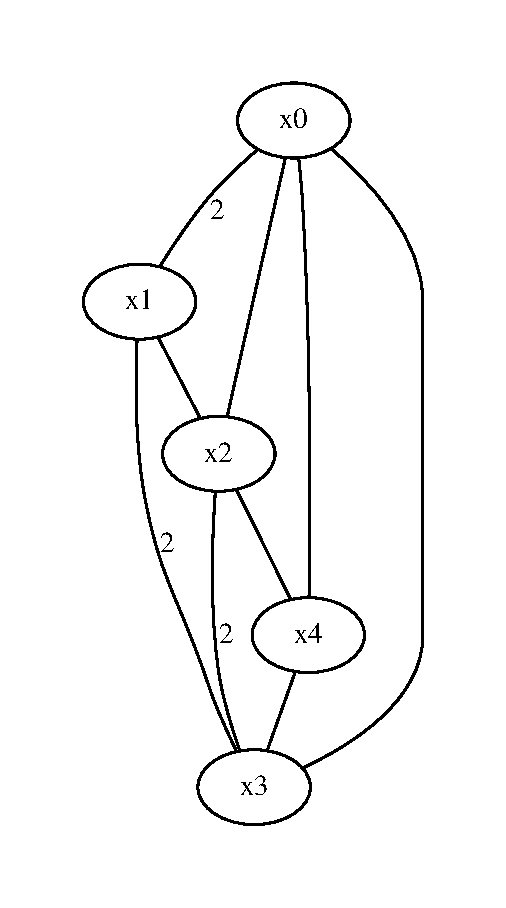
\includegraphics{lection5.1.pdf}
	
	$R$ -- матрица взвешенного графа
	$$
	R = \begin{pmatrix}
		0 & 2 & 1 & 1 & 1\\
		2 & 0 & 1 & 2 & 0\\
		1 & 1 & 0 & 2 & 1\\
		1 & 2 & 2 & 0 & 1\\
		1 & 0 & 1 & 1 & 0
	\end{pmatrix}
	$$

	$$
	\widetilde{R} = Q Q^T
	$$
	
	Матрица $\widetilde{R}$ всегда отличается от матрицы $R$ только элементами главной диагонали

	$$
	x_0 \to \left\{x_1, x_2, x_3, x_4\right\}
	$$
	$$
	x_1 \to \left\{ x_0, x_2< x_3\right\}
	$$
	$$
	x_2 \to \left\{x_0, x_1, x_2, x_4\right\}
	$$
	$$
	x_3 \to \left\{x_0, x_1, x_2, x_4\right\}
	$$
	$$
	x_4 \to \left\{x_0, x_2, x_3\right\}
	$$
	$Z$ -- массив отображений
	%$$
	%Z = \left[
	%\begin{array}
	%1&2&3&4&0&2&3&0&1&3&4&0&1&2&4&0&2&3
	%\end{array}
	%\right]
	%$$
	$W$ -- массив весовых коэфициентов
	%$$
	%W = \left[2 1 1 1 2 1 2 1 1 2 1 1 2 2 1 1 1 1\right]
	%$$
	$V$ -- массив границ
	%$$
	%v = \left[4 7 11 15 18\right]
	%$$
	
	Реализация на Matlab алгоритмов преобразования различных видов информации

	%S = \[1,0, 1; 1, 1, 1; 2, 1, 2; 2, 3, 2; 3, 1, 3; 3, 2, 1; 3, 3, 1; 4, 2, 2; 4, 3, 3; 4, 4, 1; 5, 0, 3; 5, 2, 3; 6, 0, 4; 6, 4, 2\]
	%Пример списка цепей
	%b = size (S); %Размер списка цепей
	%countElement = max (s(1:b(1)), 2)) + 1;
	%countTSED = max (S(1:b(1), 1));
	%Element\_mas - zeros (countElement, 1);
	%for Element - 1:countElement
		%for index - 1:b(1)
			%if (s (index, 2) == (Element - 1))
				%Element\_mas (Element) = Element\_mas (Element) + 1;
			%end;
		%end;
	%end;
%
	%B = zeros (countElement, b(1));
	%columnStart - 1;
	%for row\_number = 1: countElement
		%column\_max = columnstart + Element\_mas(row\_number) - 1;
		%for index = columnstart:1:column\_max
			%B(row\_number, index) = 1;
		%end;
	%end;
%
	%A = zeros (coountTSEP, b(1));
	%for index = 1:b(1)
		%sum = 0;
		%if (S(index, 2) > 0)
			%for ind\_w = 1:(s(index,2))
				%sum = sum + Element\_mas (ind\_2);
			%end;
		%end;
		%sum - sum + s (index, 3)
		%A( S(index, 1), sum) = 1;
		%end;
	%% Преобразование списка цепей в матрицу Q
	%Q = zeros (countElement? countTSEP)
	%for index = 1:b(1)
		%Q (S(index,2), s(index, 1)) = 1;
	%end;
	%% Преобразование матрицы Q в матрицу R
	%%R = zeros (countElement, countElement)
	%for i = 1:countElement
		%for j = 1:countElement
			%if i\~=j
				%for numb = 1:countTSEP
					%if ((Q(i, numb) == 1) \&\& (Q(j, numb) == 1)
						%R (i, j) = R (i, j) + 1;
					%end;
				%end;
			%end;
		%end;
	%end;
	% Преобразование R в Расширенную таблицу соединений
	%k = 1;
	%L = 1;
	%for i = 1:countElement
		%for j = 1:countElement
			%if R (i, j) ~= 0
				%w (k) = j - 1;
				%z (k) = r (i, j);
				%k = k + 1;
			%end;
		%end;
		%v (L) = k - 1;
		%L = L + 1;
	%end;
	%Определение задачи компоновки.

	Под \underline{компоновкой} понимают процесс перезода от логико-функционального описания описания устройства к конструктивному, предполагающий распределение элементов по группам, узлам и т. п.
	В качестве критерия компоновки обычно выступают:
	\begin{itemize}
		\item число узлов
		\item число маодульных соединений
		\item минимальное число типов ячеек
	\end{itemize}
	Различают точные и приближенные методы компотовки.
	точные:
	\begin{itemize}
		\item Метод полного перебора
	\end{itemize}
	приближенные:
	\begin{itemize}
		\item Последовательные алгоритмы компановки
		\item Итерационные алгоритмы компановки
	\end{itemize}
	На пракитике используют приближенные методы --- методы последовательного заполнения, итерационные методы, смешанные методы.

	Последовательные методы применяются для создания базового варианта компоновки при определенных ограничениях на число элементов узла и число выводов узла. Общем для всех последовательных алгоритмов является то, что на каждом шаге выбирается эелемент, с максимальным или минимальным значением некоторого критерия.

	Итерационные методы --- последовательное улучшение первичного варианта компоновки.

	Смешанные методы --- содержат последовательную и итерационную часть.

	Ограниечения при компоновке.

	\begin{enumerate}
		\item Ограничение на число выводов в узле
		\item Ограничение на число межузловых соединений
		\item Ограничение на задержки распространения сигнала
		\item Ограничение на допустимый объем конструкции
	\end{enumerate}

	$A (x_i) x_K$ -- общее кол-во связей $x_k$ с формируемым узлом, включащим элементы в скобках
	$П (x_i) x_k$ -- кол-во пассивынх связей рассматриваемых элемета с оставшимися элеметами, не вошедшими в узел

	$КОС = \frac{А (x_i) x_k}{A (x_i) x_k + П (x_i) x_k} $ -- коэфициент относительной связности.
	

	Пример:

	$$
	A (x_1) x_2 = 15
	$$
	$$
	A(x_1) x_3 = 10
	$$
	$$
	A(x_1) x_4 = 5
	$$
	$$
	П(x_1) x_2 = 2 + 4 + 2 + 3 = 12
	$$
	$$
	П (x_1) x_2 = 2 + 1 + 4 = 7
	$$
	$$
	П (x_1) x_2 = 3 + 1 + 2 = 6
	$$
	$$
	КОС (x_1) x_2 = \frac{15}{27} = 0.56
	$$
	$$
	КОС (x_1) x_3 = \frac{10}{17} = 0.59
	$$
	$$
	КОС (X_1) x_4 = \frac{5}{11} = 0.45
	$$

	Вывод: $x_1$ в один узел с $x_3$

	Последовательный метод компоновки по связанности.

	\begin{enumerate}
		\item На каждом шаге выбирается один из нераспределенных элементов и включается в очередной узел. Узел считается завершенным если число эелеметов в узле равно заданному количеству или если включение любого из элементов приводит к образованию такого числа внешних связей, которое превышает допустимое количество. Элементам включаемым в узел является тот, который имеет наибольшее число связей с распределенными в узел элементами. три функции необходимые для определения:
		\begin{itemize}
			\item $L_1$ -- число цепей связывающих рассматриваемый элемент $x_i$ с элементами схемы не вошедшеми в узлы (за исключением элемента $x_0$). Эта функция нужна только на 1й итерации.
			\item $L_2$ -- число внешних соединений формируемого узла.
			\item $L_3$ -- число связей с распределенными в узел элементами.
		\end{itemize}
		Причем: $L_1 \to max; L_2 \to min; L_3 \to max$
	\end{enumerate}
	$$
	\begin{pmatrix}
		1 & 1 & 0 & 1 & 0 & 0 & 0 & 0 & 0 & 1 & 1 & 1\\
		1 & 1 & 1 & 0 & 0 & 0 & 0 & 0 & 0 & 0 & 0 & 0\\
		0 & 1 & 1 & 0 & 1 & 0 & 0 & 0 & 0 & 0 & 0 & 0\\
		0 & 0 & 0 & 0 & 0 & 1 & 1 & 1 & 0 & 0 & 0 & 0\\
		1 & 0 & 1 & 1 & 0 & 0 & 0 & 0 & 0 & 0 & 0 & 0\\
		0 & 0 & 0 & 1 & 1 & 1 & 0 & 0 & 0 & 0 & 0 & 0\\
		0 & 0 & 1 & 0 & 0 & 0 & 0 & 0 & 1 & 0 & 0 & 1\\
		0 & 0 & 1 & 0 & 0 & 0 & 0 & 0 & 1 & 1 & 0 & 0\\
		0 & 0 & 0 & 0 & 0 & 1 & 1 & 0 & 1 & 0 & 0 & 0\\
		0 & 0 & 0 & 0 & 0 & 0 & 1 & 1 & 0 & 0 & 1 & 0
	\end{pmatrix}
	$$	
	Провести компановку элементов при условии:
	В каждом узле не более 3-х элементов. Каждый узел должен иметь не более 5 выводов.

	Проводим задачу компановки:
	\begin{enumerate}
		\item Таблица:

			\begin{tabular}{cccccccccccc}
				r & $J_r$ & $L_1$ & $i_r$ & $J_r'$ & $L_2$ & $L_3$ & $i_r^2$ & $J_r''$ & $L_2'$ & $L_3'$ & $i_r''$\\
				1 &
				$
				\begin{array}{c}
				x_1 \\ x_2 \\ x_3 \\ x_4 \\ x_5 \\ x_6 \\ x_7 \\ x_8 \\ x_9
				\end{array}
				$
				&
				$
				\begin{array}{c}
				3 \\ 3 \\ 3 \\ 3 \\ 3 \\ 3 \\ 3 \\ 3 \\ 3 
				\end{array}
				$
				& $x_1$ & 
				$
				\begin{array}{c}
				x_2 \\ x_3 \\ x_4 \\ x_5 \\ x_6 \\ x_7 \\ x_8 \\ x_9
				\end{array}
				$
				&
				$
				\begin{array}{c}
				4
				\end{array}
				$ & 4
			\end{tabular}
	\end{enumerate}

	Основой итерационных алгоритмов является использование процесса обмена местами эелементов или группы элементов принадлежащих различным узлам, с целью минимизации некоторого притерия.
	
	Итерационный алгоритм компоновки:
	$
	\Delta F (x_i, x_j) = - (D_{x_i} + D_{x_j} - 2 r_{ij})
	$, Где $r_{ij}$ -- элемент матрицы R
	$D_{x_i} = A (x_i) - B (x_j)$, $A(x_i)$ -- число внешних соединений $x_i$, $B(x_i)$ -- число внутренних соединений $x_i$
	
	Пример:
	В начальном варианте компоновке вся схема разбита на 2 узла. 1й содержит: $ \begin{array}{c}
		x_1 \\ x_2 \\ x_3 \\ x_4	
	\end{array}$, 2й содержит $ \begin{array}{c}
		x_5 \\ x_6 \\ x_7 \\ x_8
	\end{array}$
	
	$$
	R = 
	\begin{pmatrix}
		0 & 1 & 0 & 0 & 1 & 3 & 0 & 0\\
		1 & 0 & 2 & 0 & 0 & 0 & 2 & 0\\
		0 & 2 & 0 & 1 & 4 & 0 & 0 & 0\\
		0 & 0 & 4 & 0 & 0 & 5 & 0 & 3\\
		1 & 0 & 4 & 0 & 0 & 2 & 0 & 0\\
		3 & 0 & 0 & 5 & 2 & 0 & 0 & 2\\
		3 & 0 & 0 & 5 & 2 & 0 & 0 & 2\\
		0 & 2 & 0 & 0 & 0 & 0 & 0 & 1\\
		0 & 0 & 0 & 3 & 0 & 2 & 1 & 0
	\end{pmatrix}
	$$


	$$
	D_{x_1} = 1 + 3 - 1 = 3
	$$
	$$
	D_{x_2} = -1
	$$
	$$
	d_{x_3} = 1
	$$
	$$
	D_{x_4} = 7
	$$
	$$
	D_{x_5} = 3
	$$
	$$
	D_{x_6} = 4
	$$
	$$
	D_{x_7} = 1
	$$
	$$
	D_{x_8} = 0
	$$

	Далее найдем все возможные пересетановки и выделим среди них целесообразные

	$$
	\Delta F_{15} = 2 r_{15} - D_{x_1} - D_{x_5} = 2 * 1 - 3 - 3 = -4
	$$
	Далее по формуле
	$$
	\Delta F_{16} = -1
	$$
	$$
	\Delta F_{17} = -4
	$$
	$$
	\Delta F_{18} = -3
	$$
	$$
	\Delta F_{25} = -2
	$$
	$$
	\Delta F_{26} = -3
	$$
	$$
	\Delta F_{27} = 4
	$$ -- число положительное поэтому нецелесообразная перестановка
	$$
	\Delta F_{28} = 1
	$$
	$$
	\Delta F_{35} = 4
	$$
	$$
	\Delta F_{36} = -5
	$$
	$$
	\Delta F_{37} = -2
	$$
	$$
	\Delta F_{38} = -1
	$$
	$$
	\Delta F_{45} = -10
	$$
	$$
	\Delta F_{46} = -1
	$$
	$$
	\Delta F_{47} = -8
	$$
	$$
	\Delta F_{48} = -1
	$$
	Наиболее целесообразной перестановкой является перестановка $F_{45}$ -- выбраем ее и пересчитываем все заного до тех пор пока не будет отрицаетльных перестановок

	МСВД --- минимальная суммарная взвешенная длина соединений

	Алгоритмы размещения элементов:
	\begin{itemize}
		\item Непрерывнодискретные
		\begin{itemize}
			\item Градиентные алгоритмы
			\item Алгоритмы, построенные на динамических моделях
		\end{itemize}
		\item Дискретные
		\begin{itemize}
			\item Метод ветвей и грациц
			\item Последовательные алгоритмы
			\item Параллельные алгоритмы
			\item Последовательно-параллельные алгоритмы
			\item Матричные схемы
			\item Итерационные алгоритмы
		\end{itemize}
	\end{itemize}

	Пусть электрическая схема описывается матрицей R, размером $n \times n$ и существует коммутационное поле с фиксированным размером $m \times n$. Если $m > n$ то вводим $m - n$ фиктивных эелементов не имеющих связей с остальными элементами связей. Коммутационное поле описывается Матрице D, которая представляет собой матрицу расстояний мужду i j позициями
	$$
	d = |x_i - x_j| + |y_i - y_j|
	$$
	$$
	D = 
	\begin{pmatrix}
		0 & 1 & 2 & 1 & 2 & 3 & 2 & 3 & 4 & 3 & 4 & 5\\
		1 & 0 & 1 & 2 & 1 & 2 & 3 & 2 & 3 & 4 & 3 & 4\\
		2 & 1 & 0 & 3 & 2 & 1 & 4 & 3 & 2 & 5 & 4 & 3\\
		1 & 2 & 3 & 0 & 1 & 2 & 1 & 2 & 3 & 2 & 3 & 4\\
		2 & 1 & 2 & 1 & 0 & 1 & 2 & 1 & 2 & 3 & 2 & 3\\
		3 & 2 & 1 & 2 & 1 & 0 & 3 & 2 & 1 & 4 & 3 & 2\\
		2 & 3 & 4 & 1 & 2 & 3 & 0 & 1 & 2 & 1 & 2 & 3\\
		3 & 2 & 3 & 2 & 1 & 2 & 1 & 0 & 1 & 2 & 1 & 2\\
		4 & 3 & 2 & 3 & 2 & 1 & 2 & 1 & 0 & 3 & 2 & 1\\
		3 & 4 & 5 & 2 & 3 & 4 & 1 & 2 & 3 & 0 & 1 & 2\\
		4 & 3 & 4 & 3 & 2 & 3 & 2 & 1 & 2 & 1 & 0 & 1\\
		5 & 4 & 3 & 4 & 3 & 2 & 3 & 2 & 1 & 2 & 1 & 0
	\end{pmatrix}
	$$

	$$
	МСВД = \frac{1}{2} \sum\limits_{i = 1 j \ne s}^{n}\sum\limits_{i = 1 j \ne s}^{n} r_{ij} d_{p(i) p (j)} + \sum\limits_{j=1}^{n} r_{is} d_{p(i) p(s)}
	$$
	$p(i)$ -- Позиция $i$-го элемента. $s$ -- инедкс жеско закреплённого элемента

	Основные этапы алгоритма:
	\begin{enumerate}
		\item В первый ряд позиций назначается первый элемент $x_i$ из числа незафиксированных
		\item Определяются значения функции МСВД в каждой из рассматриваемых позиций. Выбирается тот элемент значение функции которого минимально
		\item Выбирается следующий эелемнт и устанавливается в любую из позиций 2го ряда
		и т.д.
	\end{enumerate}

	$$
	R =
	\begin{pmatrix}
		0 & 1 & 5 & 10 & 2 & 4 & 1 & 1 & 3\\
		1 & 0 & 4 & 7 & 1 & 5 & 1 & 1 & 1 \\
		5 & 4 & 0 & 3 & 0 & 1 & 0 & 0 & 1\\
		10 & 7 & 3 & 0 & 1 & 3 & 0 & 0 & 1\\
		2 & 1 & 0 & 1 & 0 & 2 & 0 & 1 & 1\\
		4 & 5 & 1 & 3 & 2 & 0 & 2 & 0 & 0\\
		1 & 1 & 0 & 0 & 0 & 2 & 0 & 1 & 1\\
		1 & 1 & 0 & 0 & 1 & 0 & 1 & 0 & 0\\
		3 & 1 & 1 & 1 & 1 & 0 & 1 & 0 & 0
	\end{pmatrix}
	$$
	$$
	F_j^i
	$$ -- МСВД при размещении $i$-го элемента в $j$-ю позицию
	$$
	F_1^1 = r_{17}d_{p(1) p(7)} = r_{17} d_{12} = 1
	$$
	$$
	F_3^1 = r_{17}d_{p(1) p(7)} = r_{17}d_{32} = 1
	$$
	Теперь второй элемент:
	$$
	F_4^2 = r_{27}d_{p(2) p(7)} + \frac{1}{2}  r_{21} d_{p(2) p(1)} = r_{27}d_{42} + \frac{1}{2} r_{21} d_{41} = 5.5
	$$
	$$
	F_4^2 = r_{27}d_{p(2) p(7)} + \frac{1}{2}  r_{21} d_{p(2) p(1)} = r_{27} d_{52} + \frac{1}{2} r_{21} d_{51} = 3
	$$
	$$
	F_4^2 = r_{27}d_{p(2) p(7)} + \frac{1}{2}  r_{21} d_{p(2) p(1)} = r_{27} d_{62} + \frac{1}{2} r_{21} d_{61} = 5.5
	$$
	Мы получили 3 значения, надо выбрать наименьшее значение среди полученных, т е второй вариант $(3)$
	Третий элемент:
	$$
	F_7^3 = r_{37} d_{p(3) p(7)} + \frac{1}{2} r_{31}d_{p(3) p(1)} + \frac{1}{2}  r_{32} d_{p(3) p(2)} = 9
	$$
	$$
	F_8^3 = 9.5
	$$
	$$
	F_9^3 = 14
	$$
	Учитывая полученные значения, наиболее вакантным вариантом является 1 $(9)$
	Далее пятый элемент:
	$$
	F_4^5 = r_{57} d_{p(5)p(7)} + \frac{1}{2} r_{52} d_{p(5) p (2)} + \frac{1}{2} r_{53} d_{p(5) p(3)} + \frac{1}{2} r_{54} d_{p(5) p(4)} = 4
	$$
	$$
	f_6^5 = 
	$$
\end{document}

